\documentclass[landscape,final,paperwidth=24in,paperheight=36in]{baposter}

\usepackage{calc}
\usepackage{graphicx}
\usepackage{amsmath}
\usepackage{amssymb}
\usepackage{relsize}
\usepackage{multirow}
\usepackage{rotating}
\usepackage{bm}
\usepackage{url} 

\usepackage{amsthm} 
\usepackage{amssymb}
\usepackage{amsmath}

\usepackage{graphicx}

\newtheorem{corolario}{Corolario}
\newtheorem{conjetura}{Conjetura}
\newtheorem*{ejemplo*}{Ejemplo}
\newtheorem*{definicion*}{Definici\'on}
\newtheorem{definicion}{Definici\'on}
\newtheorem{proposicion}{Proposici\'on}
\newtheorem{lema}{Lema}
\newtheorem{teorema}{Teorema}

\usepackage{graphicx}
\usepackage{multicol}

%\usepackage{times}
%\usepackage{helvet}
%\usepackage{bookman}
\usepackage{palatino}

\newcommand{\captionfont}{\footnotesize}

\graphicspath{{images/}{../images/}}
\usetikzlibrary{calc}

\newcommand{\SET}[1]  {\ensuremath{\mathcal{#1}}}
\newcommand{\MAT}[1]  {\ensuremath{\boldsymbol{#1}}}
\newcommand{\VEC}[1]  {\ensuremath{\boldsymbol{#1}}}
\newcommand{\Video}{\SET{V}}
\newcommand{\video}{\VEC{f}}
\newcommand{\track}{x}
\newcommand{\Track}{\SET T}
\newcommand{\LMs}{\SET L}
\newcommand{\lm}{l}
\newcommand{\PosE}{\SET P}
\newcommand{\posE}{\VEC p}
\newcommand{\negE}{\VEC n}
\newcommand{\NegE}{\SET N}
\newcommand{\Occluded}{\SET O}
\newcommand{\occluded}{o}

%%%%%%%%%%%%%%%%%%%%%%%%%%%%%%%%%%%%%%%%%%%%%%%%%%%%%%%%%%%%%%%%%%%%%%%%%%%%%%%%
%%%% Some math symbols used in the text
%%%%%%%%%%%%%%%%%%%%%%%%%%%%%%%%%%%%%%%%%%%%%%%%%%%%%%%%%%%%%%%%%%%%%%%%%%%%%%%%

%%%%%%%%%%%%%%%%%%%%%%%%%%%%%%%%%%%%%%%%%%%%%%%%%%%%%%%%%%%%%%%%%%%%%%%%%%%%%%%%
% Multicol Settings
%%%%%%%%%%%%%%%%%%%%%%%%%%%%%%%%%%%%%%%%%%%%%%%%%%%%%%%%%%%%%%%%%%%%%%%%%%%%%%%%
\setlength{\columnsep}{1.5em}
\setlength{\columnseprule}{0mm}

%%%%%%%%%%%%%%%%%%%%%%%%%%%%%%%%%%%%%%%%%%%%%%%%%%%%%%%%%%%%%%%%%%%%%%%%%%%%%%%%
% Save space in lists. Use this after the opening of the list
%%%%%%%%%%%%%%%%%%%%%%%%%%%%%%%%%%%%%%%%%%%%%%%%%%%%%%%%%%%%%%%%%%%%%%%%%%%%%%%%
\newcommand{\compresslist}{%
\setlength{\itemsep}{1pt}%
\setlength{\parskip}{0pt}%
\setlength{\parsep}{0pt}%
}

%%%%%%%%%%%%%%%%%%%%%%%%%%%%%%%%%%%%%%%%%%%%%%%%%%%%%%%%%%%%%%%%%%%%%%%%%%%%%%
%%% Begin of Document
%%%%%%%%%%%%%%%%%%%%%%%%%%%%%%%%%%%%%%%%%%%%%%%%%%%%%%%%%%%%%%%%%%%%%%%%%%%%%%

\begin{document}

%%%%%%%%%%%%%%%%%%%%%%%%%%%%%%%%%%%%%%%%%%%%%%%%%%%%%%%%%%%%%%%%%%%%%%%%%%%%%%
%%% Here starts the poster
%%%---------------------------------------------------------------------------
%%% Format it to your taste with the options
%%%%%%%%%%%%%%%%%%%%%%%%%%%%%%%%%%%%%%%%%%%%%%%%%%%%%%%%%%%%%%%%%%%%%%%%%%%%%%
% Define some colors

%\definecolor{lightblue}{cmyk}{0.83,0.24,0,0.12}
\definecolor{lightblue}{rgb}{0.145,0.6666,1}

% Draw a video
\newlength{\FSZ}
\newcommand{\drawvideo}[3]{% [0 0.25 0.5 0.75 1 1.25 1.5]
   \noindent\pgfmathsetlength{\FSZ}{\linewidth/#2}
   \begin{tikzpicture}[outer sep=0pt,inner sep=0pt,x=\FSZ,y=\FSZ]
   \draw[color=lightblue!50!black] (0,0) node[outer sep=0pt,inner sep=0pt,text width=\linewidth,minimum height=0] (video) {\noindent#3};
   \path [fill=lightblue!50!black,line width=0pt] 
     (video.north west) rectangle ([yshift=\FSZ] video.north east) 
    \foreach \x in {1,2,...,#2} {
      {[rounded corners=0.6] ($(video.north west)+(-0.7,0.8)+(\x,0)$) rectangle +(0.4,-0.6)}
    }
;
   \path [fill=lightblue!50!black,line width=0pt] 
     ([yshift=-1\FSZ] video.south west) rectangle (video.south east) 
    \foreach \x in {1,2,...,#2} {
      {[rounded corners=0.6] ($(video.south west)+(-0.7,-0.2)+(\x,0)$) rectangle +(0.4,-0.6)}
    }
;
   \foreach \x in {1,...,#1} {
     \draw[color=lightblue!50!black] ([xshift=\x\linewidth/#1] video.north west) -- ([xshift=\x\linewidth/#1] video.south west);
   }
   \foreach \x in {0,#1} {
     \draw[color=lightblue!50!black] ([xshift=\x\linewidth/#1,yshift=1\FSZ] video.north west) -- ([xshift=\x\linewidth/#1,yshift=-1\FSZ] video.south west);
   }
   \end{tikzpicture}
}

\hyphenation{resolution occlusions}
%%
\begin{poster}%
  % Poster Options
  {
  % Show grid to help with alignment
  grid=false,
  % Column spacing
  colspacing=1em,
  columns=2,
  % Color style
  bgColorOne=gray,
  bgColorTwo=white,
  borderColor=black,
  headerColorOne=white,
  headerColorTwo=lightblue,
  headerFontColor=black,
  boxColorOne=white,
  boxColorTwo=lightblue,
  % Format of textbox
  textborder=roundedleft,
  % Format of text header
  eyecatcher=true,
  headerborder=closed,
  headerheight=0.1\textheight,
 % textfont=\sc
  headershape=roundedright,
  headershade=shadelr,
  headerfont=\textsc, %Sans Serif,
  textfont=\scriptsize{\setlength{\parindent}{1.5em}},
  boxshade=plain,
%  background=shade-tb,
  background=plain,
  linewidth=2pt
  }
  % Eye Catcher
  {
\includegraphics[height=8em,keepaspectratio=true]{images/logo_uprrp}} 
  % Title
  {\bf {\LARGE Generating Families of Permutation Trinomials}}
  % Authors
  {\color{white}{{\normalsize Christian A. Rodr\'{\i}guez; Alex D. Santos \\ Department of Computer Science, \\ University of Puerto Rico, Rio Piedras Campus}}}
  % University logo
  {% The makebox allows the title to flow into the logo, this is a hack because of the L shaped logo.
    
  }

%%%%%%%%%%%%%%%%%%%%%%%%%%%%%%%%%%%%%%%%%%%%%%%%%%%%%%%%%%%%%%%%%%%%%%%%%%%%%%
%%% Now define the boxes that make up the poster
%%%---------------------------------------------------------------------------
%%% Each box has a name and can be placed absolutely or relatively.
%%% The only inconvenience is that you can only specify a relative position 
%%% towards an already declared box. So if you have a box attached to the 
%%% bottom, one to the top and a third one which should be in between, you 
%%% have to specify the top and bottom boxes before you specify the middle 
%%% box.
%%%%%%%%%%%%%%%%%%%%%%%%%%%%%%%%%%%%%%%%%%%%%%%%%%%%%%%%%%%%%%%%%%%%%%%%%%%%%%
    %
    % A coloured circle useful as a bullet with an adjustably strong filling
    \newcommand{\colouredcircle}{%
      \tikz{\useasboundingbox (-0.2em,-0.32em) rectangle(0.2em,0.32em); \draw[draw=black,fill=lightblue,line width=0.03em] (0,0) circle(0.18em);}}

%%%%%%%%%%%%%%%%%%%%%%%%%%%%%%%%%%%%%%%%%%%%%%%%%%%%%%%%%%%%%%%%%%%%%%%%%%%%%%
\headerbox{Problema}{name=problem,column=1,row=0}{
  %%%%%%%%%%%%%%%%%%%%%%%%%%%%%%%%%%%%%%%%%%%%%%%%%%%%%%%%%%%%%%%%%%%%%%%%%%%%%%
  
Estudiar el conjunto de valores de polinomios de la forma {\large $$F_{a,b}(X) = X(X^{\frac{q-1}{d_1}} + aX^{\frac{q-1}{d_2}} +b)$$} sobre cuerpos finitos $\mathbb{F}_q$ y determinar condiciones en $a,b$ tal que el polinomio es un polinomio de permutaci\'on.


}\label{Problem}

%%%%%%%%%%%%%%%%%%%%%%%%%%%%%%%%%%%%%%%%%%%%%%%%%%%%%%%%%%%%%%%%%%%%%%%%%%%%%%
  \headerbox{Resumen}{name=abstract,column=0}{
%%%%%%%%%%%%%%%%%%%%%%%%%%%%%%%%%%%%%%%%%%%%%%%%%%%%%%%%%%%%%%%%%%%%%%%%%%%%%%

Dado un trinomio de la forma $f_{a,b}(X)=X^r( X^{\frac{q-1}{d_1}}+aX^{\frac{q-1}{d_2}}+b )$ sobre un cuerpo finito $\mathbb{F}_q$ con un conjunto de valores de tama\~{n}o  $s$, \linebreak constru\'{\i}mos otros $d$ trinomios en $\mathbb{F}_q$ con el mismo tama\~{n}o de conjunto de valores, donde $d=mcm(d_1, d_2)$. En particular, dado un polinomio de permutaci\'{o}n de la forma $f_{a,b}$, constru\'{\i}mos $d$ otros polinomios de permutaci\'{o}n en $\mathbb{F}_q$. Tambi\'{e}n generamos secuencias $P_{q^{m_1}}, P_{q^{m_2}}, \cdots,$ donde $P_{q^{m_i}}$ es un polinomio de permutaci\'{o}n en $\mathbb{F}_{q^{m_i}}$.
   

 }\label{Abstract}

%%%%%%%%%%%%%%%%%%%%%%%%%%%%%%%%%%%%%%%%%%%%%%%%%%%%%%%%%%%%%%%%%%%%%%%%%%%%%%
  \headerbox{Resultados - Permutaci\'on}{name=contribution,column=1,below=problem}{
%%%%%%%%%%%%%%%%%%%%%%%%%%%%%%%%%%%%%%%%%%%%%%%%%%%%%%%%%%%%%%%%%%%%%%%%%%%%%%


\begin{proposicion}
  
  $|[F_{a, b}]| = mcm(d_1,d_2)$.

\end{proposicion}

Dado un polinomio podemos construir otros $mcm(d_1, d_2)$ polinomios con conjunto de valores de la misma cardinalidad:
$$(\alpha^{2}, \alpha^{26}), (\alpha^{8}, \alpha^{8}), (\alpha^{14}, \alpha^{26}), (\alpha^{20}, \alpha^{8}), (\alpha^{26}, \alpha^{26}), (\alpha^{32}, \alpha^{8})$$
  
    \begin{teorema}\label{laprop}
    El n\'umero de polinomios de la forma $F_{a, b}(X)$ con $|V_{a, b}| = n$ es un m\'ultiplo de $mcm(d_1,d_2)$.
  \end{teorema}

Un resultado directo del Teorema~\ref{laprop} es el caso particular cuando $|V_{a, b}| = q$, esto implica que tenemos polinomios de permutaci\'on. La construcci\'on establecida anteriormente nos provee una manera de construir familias de polinomios de permutaci\'on.

  \begin{corolario}
    El n\'umero de polinomios de permutaci\'on de la forma $F_{a, b}(X)$ es un m\'ultiplo de $mcm(d_1,d_2)$.
  \end{corolario}

  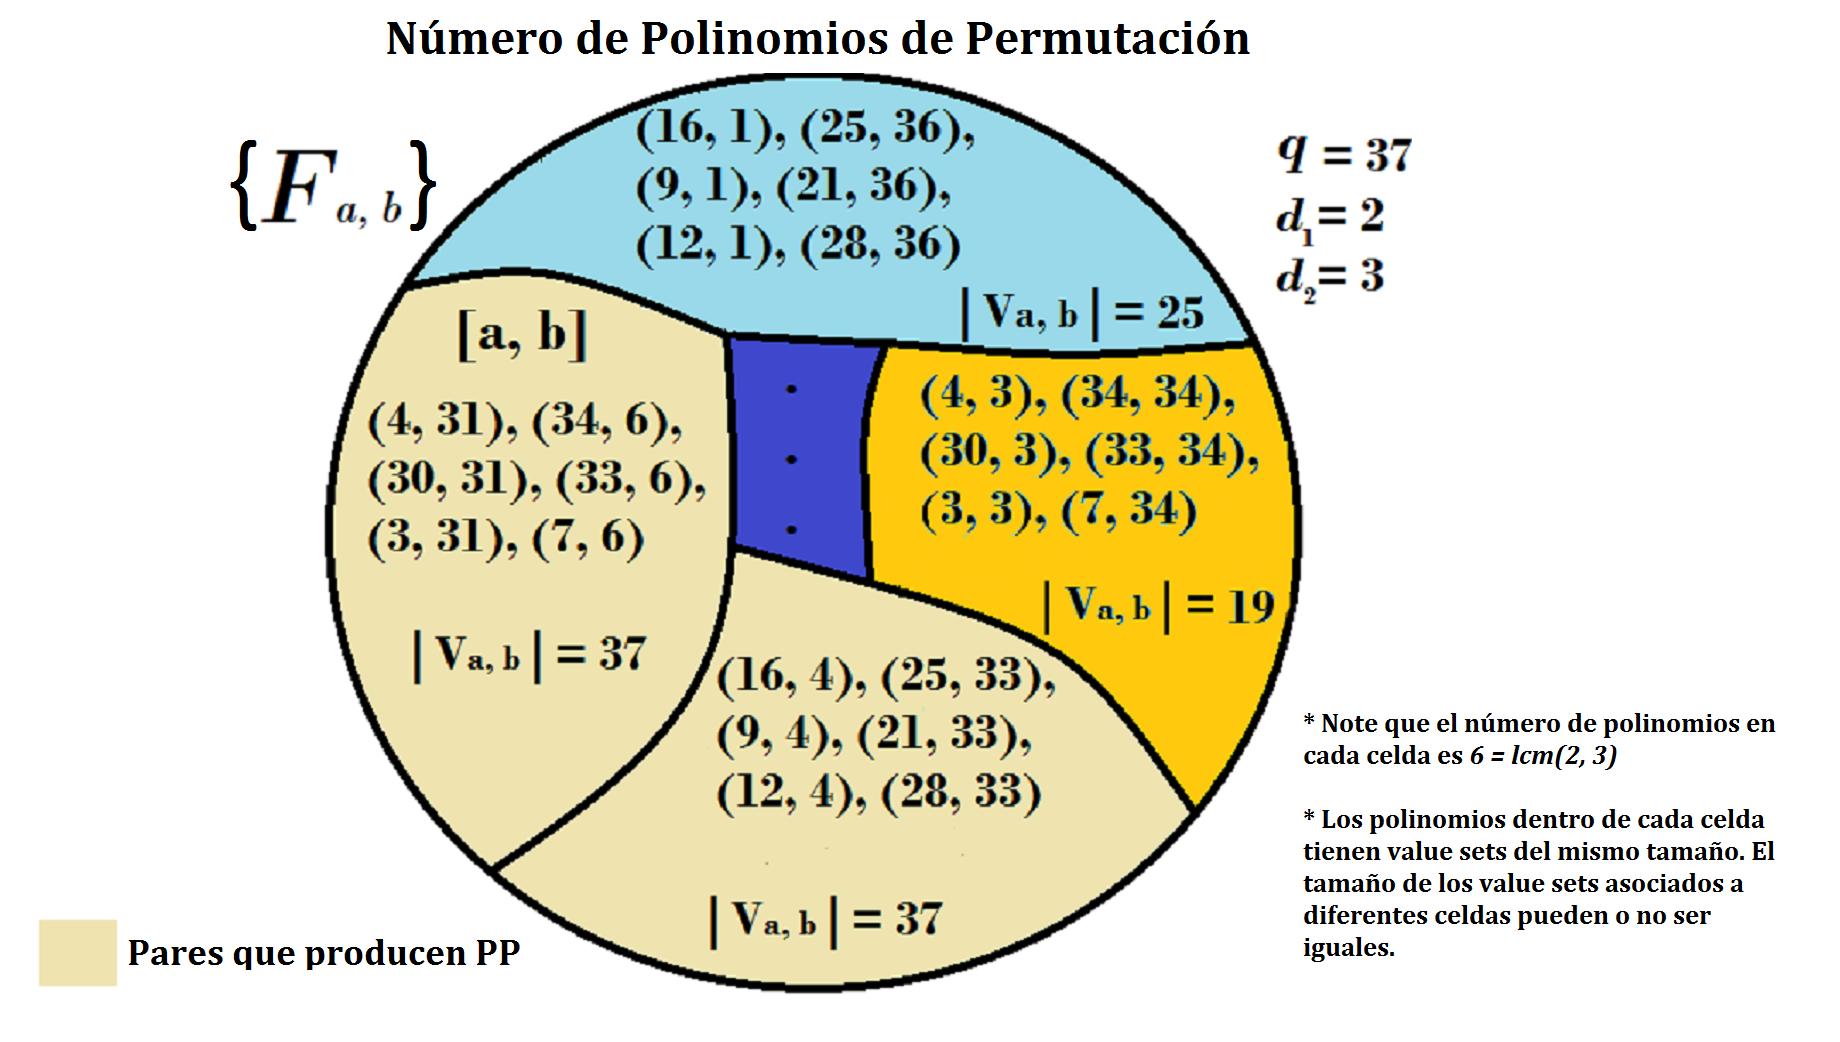
\includegraphics[width=8cm, height=5cm]{clases-espa}

}\label{Results}

%%%%%%%%%%%%%%%%%%%%%%%%%%%%%%%%%%%%%%%%%%%%%%%%%%%%%%%%%%%%%%%%%%%%%%%%%%%%%%
\headerbox{Trabajo Futuro}{name=future,column=1,below=contribution}{
  %%%%%%%%%%%%%%%%%%%%%%%%%%%%%%%%%%%%%%%%%%%%%%%%%%%%%%%%%%%%%%%%%%%%%%%%%%%%%%
    \begin{itemize}
    \item Encontrar condiciones suficientes y necesarias tal que $V_{a,b} = \mathbb{F}_q$ y $V_{a,b}$ sea de cardinalidad m\'{\i}nima.
    \item Generalizar los resultados a polinomios con m\'as t\'erminos y con exponentes no divisores de $q-1$: $f_{a,b}(X) = X^r(X^{d_1} + aX^{d_2} +b)$.
  \end{itemize}
}\label{Applications}

%%%%%%%%%%%%%%%%%%%%%%%%%%%%%%%%%%%%%%%%%%%%%%%%%%%%%%%%%%%%%%%%%%%%%%%%%%%%%%
  \headerbox{Preliminares}{name=preliminaries,column=0,below=abstract}{
%%%%%%%%%%%%%%%%%%%%%%%%%%%%%%%%%%%%%%%%%%%%%%%%%%%%%%%%%%%%%%%%%%%%%%%%%%%%%%

\begin{definicion*}
  Una \textbf{permutaci\'on} de un conjunto $A$ es un ordenamiento de los elementos de $A$. Una funci\'on $f: A \rightarrow A$ nos da una permutaci\'on de $A$ si y solo si $f$ es uno a uno y sobre.
\end{definicion*}

\begin{definicion*}
  Un \textbf{cuerpo finito} $\mathbb{F}_{q}$, $q=p^r$, $p$ primo, es un conjunto con $q=p^r$ elementos.
\end{definicion*}

\begin{definicion*}
  Una \textbf{ra\'{\i}z primitiva} $\alpha \in \mathbb{F}_q$ es un generador del grupo multiplicativo $\mathbb{F}_{q}^{*}$.
\end{definicion*}

\begin{ejemplo*}
  Considere el cuerpo finito $\mathbb{F}_{7}$. Tenemos que: $3^1 = 3, 3^2 = 2, 3^3 = 6, 3^4 = 4, 3^5 = 5, 3^6 = 1$, entonces $3$ es una ra\'{\i}z primitiva de $\mathbb{F}_{7}$.
\end{ejemplo*}

\begin{definicion*}
  Sea $f(x)$ un polinomio definido sobre $\mathbb{F}_{q}$. El \textbf{conjunto de valores} de $f$ esta definido por $V_{f} = \left\{f(a) \mid a \in \mathbb{F}_{q} \right\}$.
\end{definicion*}

Note que un polinomio $f(x)$ definido en $\mathbb{F}_{q}$ es un polinomio de permutaci\'on si y solo si $V_{f} = \mathbb{F}_{q}$.

}\label{Preliminaries}

%%%%%%%%%%%%%%%%%%%%%%%%%%%%%%%%%%%%%%%%%%%%%%%%%%%%%%%%%%%%%%%%%%%%%%%%%%%%%%
\headerbox{Aplicaciones}{name=applications,column=0,below=preliminaries}{
  %%%%%%%%%%%%%%%%%%%%%%%%%%%%%%%%%%%%%%%%%%%%%%%%%%%%%%%%%%%%%%%%%%%%%%%%%%%%%%
 \begin{itemize}

 \item El operador de encripci\'on de algunos sistemas de encripci\'on es una permutaci\'on de un cuerpo finito $\mathbb{F}_{q}$ y necesita ser computado eficientemente. Si expresamos ese operador en t\'erminos de un polinomio, computarlo es simple y eficiente.

 \item Polinomios con conjuntos de valores m\'{\i}nimos est\'an relaci\'onados a curvas con un n\'umero grande de puntos racionales.  

 \end{itemize}
}\label{Applications}

%%%%%%%%%%%%%%%%%%%%%%%%%%%%%%%%%%%%%%%%%%%%%%%%%%%%%%%%%%%%%%%%%%%%%%%%%%%%%%
  \headerbox{Resultados - conjuntos de valores}{name=valuesets,column=0, below=applications, above=bottom}{
%%%%%%%%%%%%%%%%%%%%%%%%%%%%%%%%%%%%%%%%%%%%%%%%%%%%%%%%%%%%%%%%%%%%%%%%%%%%%%

Definimos una relaci\'on para construir clases de equivalencia de polinomios con conjuntos de valores de la misma cardinalidad.


\begin{definicion}\label{relaci\'on}

  Sean $a = \alpha^i, b = \alpha^j$, donde $\alpha$ es una ra\'{\i}z primitiva en $\mathbb{F}_q$, y $\sim$ una relaci\'on en $\mathbb{F}_q^* \times \mathbb{F}_q^*$ definida por: $(a,b) \sim (a', b')$ 

  $\Longleftrightarrow a' = \alpha^{i+h(\frac{q-1}{d_1} - \frac{q-1}{d_2})}, b' = \alpha^{j+h(\frac{q-1}{d_1})}$, donde $h \in \mathbb{Z}$.

\end{definicion}

  \begin{ejemplo*}
    Sean $q = 13, d_1 = 2, d_2 = 3$, entonces tenemos $\alpha = 2$ y $a = 2^2 = 4, b = 2^3 = 8$. Ahora $(a,b) \sim (a',b')$ si y solo si
    $a' = \alpha^{2+2h}, b' = \alpha^{3+6h}$. Por ejemplo $(2^2,2^3) \sim (2^{2+2},2^{3+6})$.
  \end{ejemplo*}

\begin{lema}
  
  La relaci\'on $\sim$ en Def~\ref{relaci\'on} es una relaci\'on de equivalencia en $\mathbb{F}_q^* \times \mathbb{F}_q^*$.

\end{lema}

  El Lema 1 induce una relaci\'on de equivalencia en el conjunto de polinomios de la forma $F_{a,b}(X) = X(X^{\frac{q-1}{d_1}} + aX^{\frac{q-1}{d_2}} +b)$ con clases de equivalencia $[F_{a,b}] = [F_{\alpha^i, \alpha^j}] = \left\{\ F_{a',b'} | a' = \alpha^{i+h(\frac{q-1}{d_1} - \frac{q-1}{d_2})}, b' = \alpha^{j+h(\frac{q-1}{d_1})} \right\}$.

  Esto provee una construcci\'{o}n para polinomios con conjuntos de valores de la misma cardinalidad.
\begin{teorema}
  
  Suponer que $F_{a,b} \sim F_{a',b'}$ donde $\sim$ es la relaci\'on de equivalencia en el Lema 1. Entonces $|V(F_{a,b})| = |V(F_{a',b'})|$.

\end{teorema}
   

 }\label{valuesets}





%%%%%%%%%%%%%%%%%%%%%%%%%%%%%%%%%%%%%%%%%%%%%%%%%%%%%%%%%%%%%%%%%%%%%%%%%%%%%%
  \headerbox{Referencias}{name=references,column=1,above=bottom,below=future}{
%%%%%%%%%%%%%%%%%%%%%%%%%%%%%%%%%%%%%%%%%%%%%%%%%%%%%%%%%%%%%%%%%%%%%%%%%%%%%%
  \begingroup
  \renewcommand{\section}[2]{}%
   \begin{thebibliography}{}
      \bibitem{main} Panario, D., Mullen, G., \textit{Handbook of Finite Fields}. CRC Press (2013).
      \bibitem{main} Wan, D., Lidl, R. \textit{Permutation Polynomials of the Form $x^{r}f(x^{\frac{q-1}{d}})$ and Their Group Structure}. Mh. Math. 112, 149-163 (1991).
      \bibitem{main} Borges, H., Conceicao R. \textit{On the characterization of minimal conjunto de valores polynomial}. Journal of Number Theory 133 (2013) 2021-2035.
    \end{thebibliography}
   \endgroup
  }\label{References}

\end{poster}

\end{document}
